\documentclass[12pt, centerh1]{article}
\textwidth=165mm \headheight=0mm \headsep=10mm \topmargin=0mm
\textheight=220mm %\footskip=1.5cm
\oddsidemargin=0mm
%\documentclass[12pt,letterpaper]{article}
%\usepackage[margin=1in]{geometry}
\RequirePackage[colorlinks,citecolor=blue,urlcolor=blue]{hyperref}
\usepackage{amsmath, amssymb,natbib}
%\usepackage[mathscr]{euscript}
%\usepackage{mathrsfs}
\usepackage{graphicx,bm}
\usepackage{color}
\usepackage{subcaption}
 \usepackage[table]{xcolor}
\usepackage{longtable}
\usepackage{amsthm}
\usepackage[mathscr]{euscript}
\usepackage{relsize}
\newcolumntype{P}[1]{>{\centering\arraybackslash}p{#1}}
\usepackage{rotating}
\usepackage{eurosym}
\usepackage{colonequals}
\usepackage{bbm}

\usepackage{listings}


\lstset{language=R}  
\DeclareMathOperator*{\argmax}{argmax}
\DeclareMathOperator*{\argmin}{argmin}

\newcommand{\MM}{\bm{M}}
\newcommand{\MV}{\bm{V}}
\newcommand{\MU}{\bm{U}}
\newcommand\ddfrac[2]{\frac{\displaystyle #1}{\displaystyle #2}}
\newcommand\fancyV{\mathcal{V}}
\newcommand\fancyA{\mathcal{A}}
\newcommand{\tupsi}{\bm{\upsilon}}
\newtheorem{theorem}{Theorem}
 
%\usepackage{titling}
%\usepackage{lipsum}

\newcommand{\bmt}{\bm{\theta}}
\newcommand{\bmx}{\bm{x}}
\newcommand{\bmX}{\bm{X}}
\newcommand{\bmmu}{\bm{\mu}}
\newcommand{\bmSg}{\bm{\Sigma}}

\begin{document}
\section*{Q2}
\subsection*{a)}

The multivariate Gaussian Mixture Model is one of the most popular approaches to mixture modelling due to its  
mathematical tractability and computational feasibility. The dirchletprocess package (Ross et. al. 2020) by R incorporates the classic mixture model approach with the robustness of a Dirchlet process. The Infinite Multivariate Gaussian Mixture Model is an extension of the original finite mixture model in the following definition:
Let $\bmX$ be a random variable whose density is formulated as : 
$$f(\bmx|\bm{\vartheta}) = \sum_{g=1}^G \pi_g f(\bmx|\bm{\theta}_g) $$

Here, $ \sum_{g=1}^G \pi_g = 1 , \pi_g > 0, \forall g $. In addition, $f$ is the density of a multivariate Gaussian parametrized by $\bmt$. The density is given as:
$$ f(\bmx|\bm{\theta}_g) = \frac{1}{(2\pi)^{p/2} det(\bmSg_g)^{1/5}} \exp \left( (\bmx - \bmmu_g)\bmSg_g^{-1} (\bmx - \bmmu_g)' \right). $$. 

The Infinite Gaussian Mixture Model assumes the following assumptions:
\begin{align}
\bmmu_g &\sim Normal(\bmmu_0, \bmSg_0), \;\; \forall g \\
\bmSg_g & \sim Wish(\bm{V},q) & \\
z &\sim Categorical(\pi_1, \dots, \pi_G) \\
x &\sim Normal(\bmmu_z, \bmSg) \\
(\pi_1, \dots, \pi_G) &\sim Dirichlet(G, \alpha) \\
G  \to \infty &, \quad \text{under a Chinese Restaurant Process} 
\end{align}


Here, (5) is meant that groups of $G$ will be drawn according to a Chinese Restaurant Process in the following scheme. Let $\Pi_0$ be our general prior distribution for all parameters. Start with data points assigned to a cluster, k-means initialization should be good enough. First, for each of our $n$ observations, remove the data point from each initial cluster, and assign it to a new cluster with a probability proportional to $n_g \times f(\bmx|\bm{\theta}_g) $, or assign it to a new singleton cluster with probability proportional to $\int_{\mathcal{R}} f(\bmx|\bm{\theta}_g)\partial \Pi_0(\bm{\theta}_g)$.  This is a summary of the MCMC algorithm for the model described above. It is worth noting that for (1), a high variance is assumed to capture the means of distant clusters. In the event of having very separated clusters, priors should be selected with having a high variance. Performance is evaluated in using the Adjusted Rand index:

$$ARI = \frac{ \sum_{ij} \binom{n_{ij}}{2} - [\sum_i \binom{a_i}{2} \sum_j \binom{b_j}{2}] / \binom{n}{2} }{ \frac{1}{2} [\sum_i \binom{a_i}{2} + \sum_j \binom{b_j}{2}] - [\sum_i \binom{a_i}{2} \sum_j \binom{b_j}{2}] / \binom{n}{2} }, $$
where $a_i$ is the ith row sum, and $b_j$ is the jth column sum.  In summary, ARI can be thought of as the ``corrected for chance" of the number of object pairs that are either in the same group or in different groups, across all partitions divided by the total number of object pairs. Once the model has converged, we predict membership of the test set as 

$$\hat{z}_{ig} = \frac{\hat{\pi}_{g}  f(\bm{x}| \bm{\theta}_g)  }{ \sum_{k=1}^G \hat{\pi}_{k}  f(\bm{x}| \bm{\theta}_k) }. $$

We then take the maximum of the $\hat{z}_{ig}$ as the class membership i.e. we label the new data point according to the maximum probability an observation $i$ belongs to group $g$ across all groups 1 ,\dots , G. 


\paragraph{Stratified Bootstrapping}
For this particular dataset, we see that the number of diabetic and non-diabetic observations is unbalanced. To reduce over-fitting, I have split the dataset into training and test set according to an 80/20 split. Furthermore, The training set was bootstrapped randomly such that the number of diabetic v. non-diabetic observations were balanced totalling 285 observations in each class. This procedure is performed 50 times for each setting of the Infinite Gaussian Mixture model, each with different randomizations of the 80/20 split and the stratified bootstrapping. This type of bootstrapping was previously learned in STATS-780 in order to prevent over-fitting of models. Having balanced classes for classification reduces classification error in the test set. 

\subsection*{c)}

 Each covariate is of a different magnitude, scaling would be beneficial when training a model. Specifically, for the Infinite Gaussian Mixture Model, it is recommended to scale each covariate accordingly.
A concerning observation of a large number of pregnancies totalling to $17$ for a diabetic individual shows a large $bmi$ measurement of $40$. In general, a $bmi$ of 30 or greater is considered to be overweight.
Further research into the Pima Indian tribes show a rate of miscarriage among the women which explains the large number of pregnancies for this individual. 

\begin{figure}[!htb]
\label{pairsPlot}
\caption{Pairs plot of covariates coloured blue for diabetic and red for normal individuals with correlation coefficients in the upper triangular portion of the pairs plot.}
\includegraphics[scale=0.50]{plotgg}
\end{figure}


\begin{figure}[!htb]
\label{Priorcomp}
\centering
\caption{Comparing prior settings in relation to ARI}
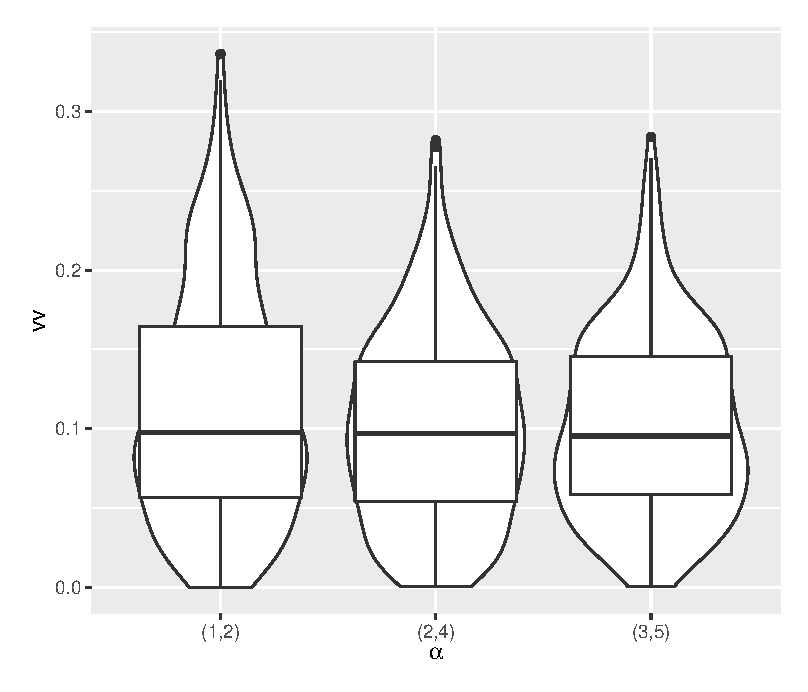
\includegraphics[scale=0.50]{priors.eps}
\end{figure}


\begin{figure}[!htb]
\label{dp_pairs}
\caption{Pairs plot of covariates coloured based on groups found with correlation coefficients in the upper triangular portion of the pairs plot.}
\includegraphics[scale=0.50]{dp_pairs}
\end{figure}



\begin{table}[!htb]
\centering
\label{tab_class}
\caption{Classification Table for a single run of bootstrapping}
\begin{tabular}{|l|cc|}
\hline
 & Normal & Diabetic \\ 
 \hline
G1 (red)     & 89     & 174      \\
G2 (brown)  & 169    & 65       \\
G3 (green)  & 23     & 45       \\
G4 (blue)  & 1      & 2000     \\
G5 (teal) & 3      & 2000     \\
G6 (magenta) & 0      & 1       \\
\hline
\end{tabular}
\end{table}


Furthermore, the pairs plot shown in Figure 1 displays the skewness of both groups and a heterogeneity within each histogram (see diagonal). In addition, the diabetic group (blue) has a multi-modal shape indicating that there may be more than one sub group within the diabetic group. Correlation coefficients between covariates remain to be relatively low (upper triangle) with $bmi$ and $skin$ having the highest correlation of $0.647$. This is to be expected as body mass index ($bmi$) measures the ratio of weight to height of body, and overweight individuals tend to have a larger tricep skin fold thickness ($skin$).  With independence between covariates established, the dataset is concluded to be of sound quality and relevant to the purpose of classifying diabetes for individuals in a population. 

When considering different prior settings for $\alpha$, we calculate the ARI across 50 different bootstraps. Custom parallel code was written for this experiment to expedite the process. Figure 2 illustrates the resultant ARIs for each bootstrap. We note that the prior has little to no effect on the predicting outcome. Due to time constraints, $\Pi_0$ priors were not considered, but can be explored in a similar fashion using the custom code. Taking a look at the specific results for one bootstrap, we have that the Infinite Gaussian Mixture model finds two groups that are closely. For a particular bootstrap we have that the algorithm finds $6$ groups. Although over-estimating the number of groups there exists a clear two groups that are a majority. Figure 3 illustrates each group given by colors. There are three main groups, and a few tertiary ones. Table 1 shows the classification table of each group (1-6) and the split between diabetic.  The first two groups (red and brown) make up a majority diabetic and majority non-diabetic. The middle group (green) is a mix of the two types, both diabetic and non-diabetic. Other groups appear to be singletons or very small groups. I believe this is a by product of the sampling method. 


\subsection*{d)}
This analysis concludes that the Infinite Gaussian Mixture Model is adept at finding clear majority groups, but is not suitable for classification. The ARI scores are very low, usually a high ARI between 0.85 - 1 is preferable for this type of work. The model results find a lot of groups than the typical diabetic. It is interesting to consider that diabetes may be a multi-type ailment. Recent research shows more than 4 types of diabetes, but answers are still unclear. 


\end{document}